\documentclass[conference]{IEEEtran}

\usepackage[T1]{fontenc}
\usepackage[utf8]{inputenc}
\usepackage[spanish, es-noshorthands, es-tabla]{babel}
\usepackage{amsmath, amssymb, bm}
\usepackage{graphicx}
\usepackage{booktabs}
\usepackage{cite}
\usepackage{url}
\usepackage[table]{xcolor}

% Valores y tablas generados por el notebook (hito2/resultados/). Se actualizan al re-ejecutarlo.
\newcommand{\resdir}{../../../hito2/resultados}
\input{\resdir/valores.tex}
\makeatletter\newcommand{\tabinput}[1]{\@@input #1 }\makeatother  % \input dentro de tabular (tras \midrule)

\graphicspath{{../../../hito2/figuras/}}
\decimalpoint

\begin{document}

\title{Integración de Modelos Cinemáticos, Diferenciales y Dinámicos para el Manipulador ABB IRB~120 (Hito~2)}

\author{
    \IEEEauthorblockN{Dayana Andrade}
    \IEEEauthorblockA{\textit{Ingeniería Mecatrónica} \\
    \textit{Universidad Católica Boliviana}\\
    Tarija, Bolivia \\
    dayana.andrade@ucb.edu.bo}
    \and
    \IEEEauthorblockN{Mirko Ayala}
    \IEEEauthorblockA{\textit{Ingeniería Mecatrónica} \\
    \textit{Universidad Católica Boliviana}\\
    Tarija, Bolivia \\
    mirko.ayala@ucb.edu.bo}
    \and
    \IEEEauthorblockN{Marcelo Navarro}
    \IEEEauthorblockA{\textit{Ingeniería Mecatrónica} \\
    \textit{Universidad Católica Boliviana}\\
    Tarija, Bolivia \\
    luis.navarro@ucb.edu.bo}
}

\maketitle

\begin{abstract}
Este documento sintetiza la implementación y validación computacional de un pipeline robótico completo para el
ABB IRB~120, desde una pose objetivo del efector hasta el torque del actuador del hombro. El robot parte de su posición
de calibración (todos los ejes en $0^\circ$) y debe alcanzar una pose objetivo $T_d$. La cinemática inversa se resuelve
de forma analítica por el método de Pieper, con enumeración de las ocho ramas y validación de cada candidato por
cinemática directa (errores del orden de $10^{-16}$). La transición se parametriza con un perfil LSPB sincronizado de
tiempo mínimo que respeta los límites del fabricante. El Jacobiano geométrico se valida contra derivadas numéricas y se
usa para estudiar, en un experimento independiente, la pérdida de rango en la singularidad de muñeca $q_5 = 0$: se
identifica la movilidad perdida y la amplificación $\lVert\dot{\mathbf{q}}\rVert \propto 1/\sin q_5$, que no implica
torque infinito. Finalmente, un modelo dinámico reducido 1R del hombro, con parámetros obtenidos de datos CAD, entrega
$\tau(t)$ separado en sus componentes inercial y gravitacional, y aproxima al modelo completo de seis grados de
libertad con un error RMS del \RMSPct\,\%.
\end{abstract}

\begin{IEEEkeywords}
Cinemática inversa, Pieper, Jacobiano, LSPB, singularidades, dinámica de manipuladores, ABB IRB~120.
\end{IEEEkeywords}

% =====================================================================================================
\section{Introducción}
El control efectivo de un manipulador industrial exige relacionar el espacio de la tarea con el espacio articular e
incorporar el tiempo para predecir los esfuerzos de los actuadores~\cite{siciliano}. El propósito de este proyecto es
construir un flujo de ingeniería que permita ir de una pose objetivo a las demandas de torque, validando cada etapa
de forma independiente. El pipeline implementado es
\begin{align*}
T_0, T_d &\xrightarrow{\text{Pieper}} \{\mathbf{q}^{(k)}\} \xrightarrow{\text{FK}} \mathbf{q}_f
\xrightarrow{\text{LSPB}} \mathbf{q}(t),\dot{\mathbf{q}}(t),\ddot{\mathbf{q}}(t)\\
&\xrightarrow{J(\mathbf{q})} \dot{\mathbf{x}}(t),\ \operatorname{rank}J \xrightarrow{\text{1R}} \tau(t).
\end{align*}
Todo el trabajo se realizó en Python con NumPy y Matplotlib, en un notebook reproducible que se ejecuta de inicio a fin
con \NChecks{} verificaciones automáticas, según la guía del curso~\cite{guia}. No se usan ROS ni solucionadores numéricos de cinemática inversa.

% =====================================================================================================
\section{Modelo del robot}
Se usa la convención Denavit--Hartenberg clásica con la tabla de Bahani \textit{et al.}~\cite{bahani}
(Tabla~\ref{tab:dh}). Sus cotas coinciden con el datasheet de ABB~\cite{abb}: en $\mathbf{q} = \mathbf{0}$ la brida
queda en $(0.374, 0, 0.630)$~m. Los límites articulares y las velocidades máximas por eje provienen del mismo
datasheet. El punto de trabajo (TCP) se ubica a 0.150~m de la brida sobre $z_6$:
$T_{TCP}(\mathbf{q}) = T_0^6(\mathbf{q})\,T_z(0.150)$. Los 0.150~m son una decisión de diseño del equipo (punto de trabajo
de la herramienta). En la dinámica solo se modela la masa de la pinza SMC MHZ2-16D (0.115~kg, hoja de datos), con su
centro de masa aproximado a 0.040~m de la brida. Mover ese centro de masa entre 0 y 0.080~m cambia el torque
gravitacional del hombro en menos de 0.07~N\,m, es decir, por debajo del 1\,\%.

\begin{table}[t]
\centering
\caption{Parámetros DH clásicos~\cite{bahani} y datos del fabricante~\cite{abb}}
\label{tab:dh}
\small
\begin{tabular}{@{}cccccc@{}}
\toprule
$i$ & $\theta_i$ & $d_i$ [m] & $a_i$ [m] & $\alpha_i$ & Rango [$^\circ$], $v_{\max}$ [$^\circ$/s]\\
\midrule
1 & $q_1$ & 0.290 & 0 & $-\pi/2$ & $\pm165$, 250\\
2 & $q_2-\pi/2$ & 0 & 0.270 & 0 & $\pm110$, 250\\
3 & $q_3$ & 0 & 0.070 & $-\pi/2$ & $-110/+70$, 250\\
4 & $q_4$ & 0.302 & 0 & $\pi/2$ & $\pm160$, 320\\
5 & $q_5$ & 0 & 0 & $-\pi/2$ & $\pm120$, 320\\
6 & $q_6+\pi$ & 0.072 & 0 & 0 & $\pm400$, 420\\
\bottomrule
\end{tabular}
\end{table}

\textbf{Pose inicial.} Se elige la \emph{posición de calibración} (sincronización) de ABB, con todos los ejes en
$0^\circ$: es la postura de referencia a la que se lleva el robot con \texttt{MoveAbsJ} y un \textit{jointtarget} de
ceros para verificar los contadores de revolución~\cite{abbcal}. Su pose es
$T_0 = FK(\mathbf{0})$: TCP en $(0.524, 0, 0.630)$~m con la herramienta orientada según $+x$. En esta postura
$q_5 = 0$, es decir, es una singularidad de muñeca.

\textbf{Pose objetivo.} Es la que entrega el docente: el TCP en $\PoseObjPos$~m con roll-pitch-yaw
$\PoseObjRPY$ ($R = R_z R_y R_x$). Es el único dato que hay que editar en el notebook.

% =====================================================================================================
\section{Metodología}

\subsection{Cinemática inversa analítica (Pieper)}
Los ejes 4, 5 y 6 se cortan en el centro de muñeca $W$, por lo que el problema se desacopla~\cite{pieper}. Primero,
$\mathbf{p}_W = \mathbf{p}_{TCP} - (0.150 + d_6)\,\mathbf{z}_6$. Luego,
$q_1 = \operatorname{atan2}(y_W, x_W)$ o $q_1 + \pi$ (brazo frente o atrás). En el plano del brazo, con
$L_3 = \sqrt{d_4^2 + a_3^2}$ y $\delta = \operatorname{atan2}(a_3, d_4)$, la ley de cosenos da
\begin{equation}
-\sin(q_3 - \delta) = \frac{D^2 - L_2^2 - L_3^2}{2L_2L_3} \equiv c,
\label{eq:cos}
\end{equation}
con dos soluciones de codo cuando $|c| \le 1$. La rama no es real si $|c| > 1$. Después,
$q_2 = \operatorname{atan2}(r, h) - \operatorname{atan2}(L_3\sin\eta,\ L_2 + L_3\cos\eta)$, con
$\eta = \pi/2 + q_3 - \delta$. Para la orientación,
$R_3^6 = (R_0^3)^TR_d = R_z(q_4)R_y(-q_5)R_z(q_6+\pi)$ es una secuencia de Euler ZYZ que se resuelve con
\texttt{atan2}; el signo de $\sin q_5$ da dos ramas de muñeca. En total hay $2\times2\times2 = 8$ ramas. Cada una se
clasifica como \emph{real}, \emph{dentro de límites} (buscando el representante $q_i + 2\pi k$ dentro del rango) y
\emph{admisible} (real, en límites y verificada por FK).

\subsection{Validación por cinemática directa y selección}
Cada rama real se reinyecta en la FK y se mide $e_p = \lVert\mathbf{p}(\mathbf{q}^{(k)}) - \mathbf{p}_d\rVert$ y el
error angular geodésico $e_R = \angle(R_d^TR(\mathbf{q}^{(k)}))$. Se acepta si $e_p < 10^{-6}$~m y
$e_R < 10^{-6}$~rad; la tolerancia en posición es diez veces menor que la repetibilidad del robot (0.01~mm). Antes de
todo, se verifica que $T_d \in SE(3)$ (última fila $[0,0,0,1]$, $R^TR = I$, $\det R = 1$). Para verificar la propia FK
se usan dos comparaciones: (i) con el modelo cinemático oficial de ROS-Industrial~\cite{rosi}, construido con
traslaciones y ejes de los planos de ABB, sin parámetros DH, que es una fuente geométrica independiente; y (ii) con el
URDF del Hito~1, que se derivó de la misma tabla DH y por eso solo comprueba la implementación.

\textbf{Criterio de selección (8 ramas $\to$ 1).} Se aplican filtros en orden: (1) rama admisible; (2)
$\sigma_{\min}(J) \ge 0.01$, que acota la amplificación de velocidad $\lVert\dot{\mathbf{q}}\rVert \le
\lVert\dot{\mathbf{x}}\rVert/\sigma_{\min}$ a 100$\times$; (3) margen de al menos $5^\circ$ respecto de cada límite
articular, para dejar espacio a los límites de software y al error de seguimiento. Entre las ramas que pasan, se elige la
de menor $\lVert W(\mathbf{q} - \mathbf{q}_0)\rVert$ con $W = \operatorname{diag}(1,1,1,0.5,0.5,0.5)$: menos tiempo,
energía y volumen barrido, priorizando las juntas que mueven más masa. El $t_f$ del LSPB se informa pero no decide,
porque lo fija una sola junta y depende del supuesto de $a_{\max}$.

\subsection{Trayectoria LSPB}
Entre $\mathbf{q}_0$ y $\mathbf{q}_f$ se construye un LSPB sincronizado. Todas las juntas comparten $t_f$ y $t_b$, con
$V_i = D_i/(t_f - t_b)$ y $a_i = V_i/t_b$. El perfil tiene un arranque parabólico, un tramo de velocidad constante y
un frenado parabólico. El $t_f$ mínimo que cumple $|V_i| \le v_{\max,i}$ y $|a_i| \le a_{\max,i}$ se obtiene por
bisección. Se usa $v_{\max} = 0.25\,v_{\text{datasheet}}$ (factor de velocidad del 25\,\%). Como ABB no publica
aceleraciones articulares, se adopta el supuesto declarado $a_{\max} = v_{\max}/0.25$~s.

\subsection{Jacobiano y detección de singularidad}
Para juntas de revolución,
$J_i = [\,\mathbf{z}_{i-1}\times(\mathbf{p}_{TCP} - \mathbf{o}_{i-1});\ \mathbf{z}_{i-1}\,]$, y
$\dot{\mathbf{x}} = J(\mathbf{q})\dot{\mathbf{q}}$. Se valida de tres formas: con diferencias centrales de la FK
(usando $[\bm{\omega}]_\times = \dot RR^T$), con columnas calculadas a mano en $\mathbf{q} = \mathbf{0}$ y comparando
$J_v\dot{\mathbf{q}}$ con $d\mathbf{p}/dt$ sobre la trayectoria. El criterio central de singularidad es el rango
numérico obtenido por SVD, $J = U\Sigma V^T$, contando los $\sigma_i > 10^{-6}$. El determinante solo se usa como
complemento, mediante la factorización
\begin{equation}
\det J = L_2L_3\cos(q_3-\delta)\,r_W\cdot(-\sin q_5),
\label{eq:det}
\end{equation}
que expone las singularidades de codo, hombro ($r_W = 0$) y muñeca. En el experimento independiente se fija
$\mathbf{q} = (30^\circ, -20^\circ, 15^\circ, 40^\circ, q_5, 60^\circ)$ y se genera una secuencia de poses
$T_k = FK(\mathbf{q}_k)$ con $q_5 \to 0$. Cada pose pasa por Pieper y FK, y luego por la SVD de $J$.

\subsection{Modelo dinámico reducido (1R)}
Para un péndulo con $\theta$ medido desde la vertical inferior, $T = \tfrac12 J\dot\theta^2$ y
$V = mg\ell_c(1 - \cos\theta)$. Euler--Lagrange da
\begin{equation}
\tau = \underbrace{J\ddot\theta}_{\tau_{in}} + \underbrace{mg\ell_c\sin\theta}_{\tau_g},\qquad J = I_c + m\ell_c^2.
\label{eq:1r}
\end{equation}
El actuador modelado es la junta 2 (hombro). Los eslabones 2 a 6 y la pinza (0.115~kg) forman un único cuerpo rígido,
con las juntas 3 a 6 congeladas en $\mathbf{q}_{\text{ref}} = (\mathbf{q}_0 + \mathbf{q}_f)/2$. Los parámetros $m$,
$\ell_c$, $I_c$ y el desfase $\varphi_0$ ($\theta = q_2 + \varphi_0$) se \emph{calculan} con los datos CAD por eslabón
de Truc y Lam~\cite{truc} y el teorema de Steiner. Las entradas $q_2(t)$ y $\ddot q_2(t)$ provienen del LSPB.

% =====================================================================================================
\section{Resultados}

\subsection{Cinemática inversa y validación}
Para la pose objetivo, $\mathbf{p}_W = \PWObj$~m y $D = \DObj$~m, dentro de $[0.040, 0.580]$~m, con
$c = \CObj$. De las 8 ramas, \NReales{} son reales y \NAdm{} admisibles (Tabla~\ref{tab:ik}); para cada rama no
admisible la tabla indica qué juntas violan sus límites. % REVISAR si cambia la pose: comentar la causa principal.
Las \NRamasReales{} ramas reales de las dos poses reproducen su pose con $e_p \le \MaxEp$~m y
$e_R \le \MaxEr$~rad, y la FK por DH coincide en pose completa con el modelo oficial de ROS-Industrial (y con el URDF del Hito~1) en
302 configuraciones, con diferencias del orden de $10^{-15}$. El criterio rechaza un candidato con error de $0.01$~rad solo en $q_6$, que tiene
$e_p = 0$, y la prueba de ida y vuelta con 1000 configuraciones aleatorias recupera el $\mathbf{q}$ original en el
100\,\% de los casos. Desde $T_0$, Pieper recupera exactamente $\mathbf{q} = \mathbf{0}$, con la muñeca marcada como
singular. La Fig.~\ref{fig:ramas} muestra la geometría de las ramas del brazo y la Fig.~\ref{fig:ramas3d} el robot
completo en cada una de las 8 ramas. Con el criterio de selección se elige la rama \RamaSel{} (\RamaSelTxt):
$\sigma_{\min} = \SigmaMinQf$, margen de $\MargenQf^\circ$ al límite más cercano y costo $\CostoQf$; \NAptas{} rama(s)
pasan los filtros.

\begin{figure*}[t]
\centering
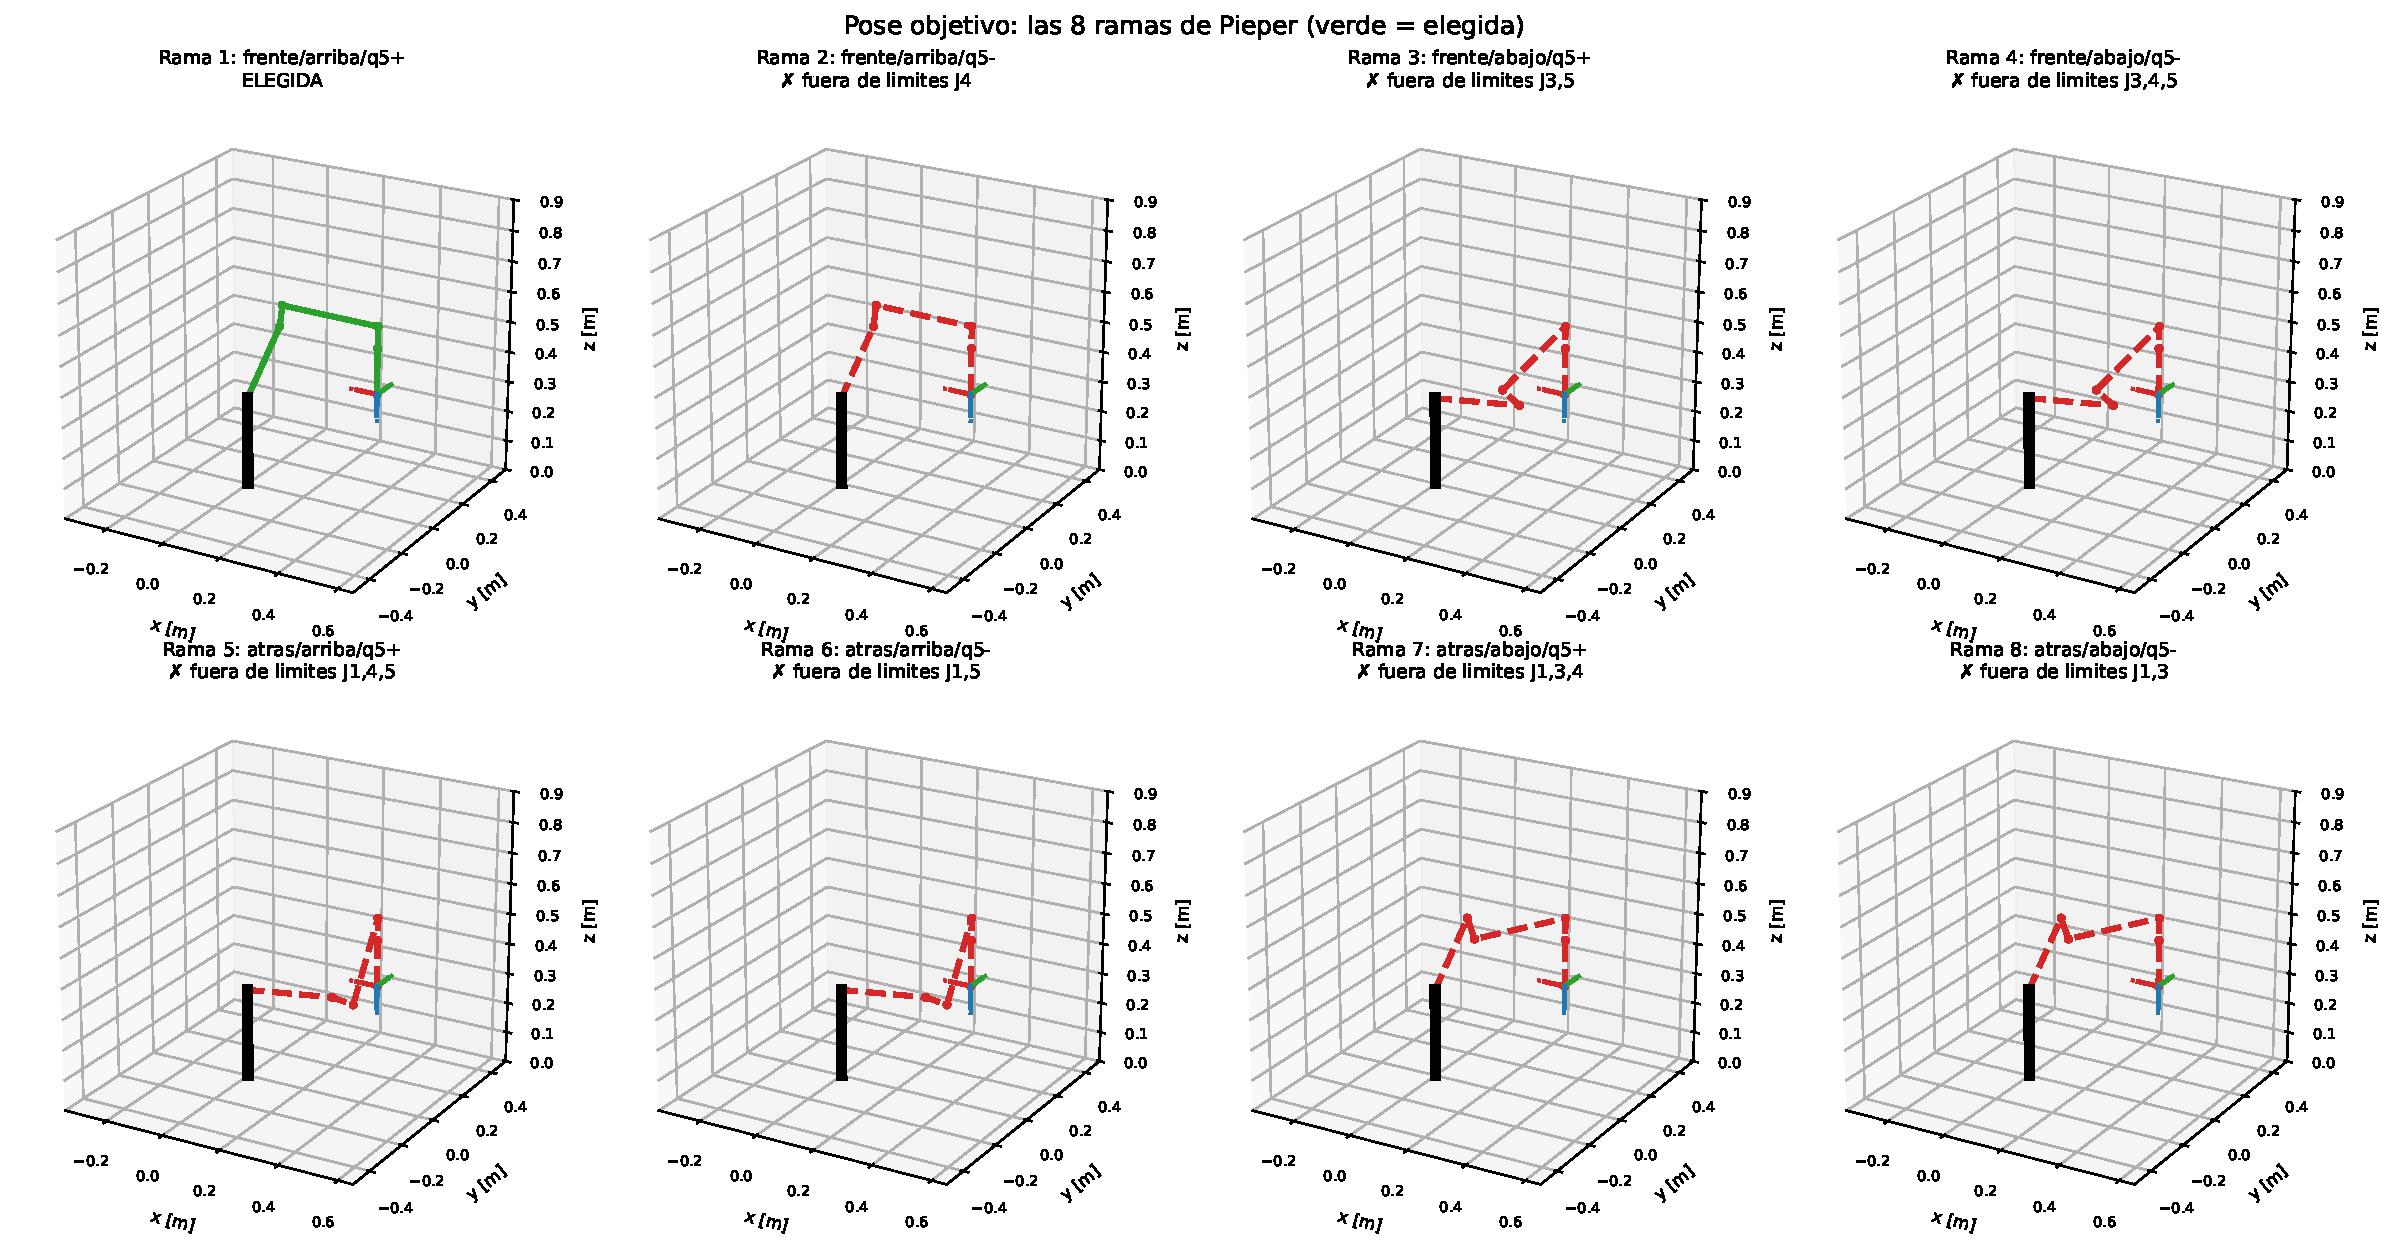
\includegraphics[width=\textwidth]{A_ocho_ramas_3d.pdf}
\caption{Las 8 ramas de Pieper para la pose objetivo. Verde: rama elegida; azul: admisible no elegida; rojo
discontinuo: existe pero viola límites (se dibuja con sus ángulos sin ajustar). En todas las ramas reales, el triedro
del TCP coincide con el triedro objetivo (punteado).}
\label{fig:ramas3d}
\end{figure*}

\begin{table}[t]
\centering
\caption{Las 8 ramas de Pieper para la pose objetivo [grados]}
\label{tab:ik}
\scriptsize
\setlength{\tabcolsep}{1.6pt}
\begin{tabular}{@{}clrrrrrrl@{}}
\toprule
$k$ & Rama & $q_1$ & $q_2$ & $q_3$ & $q_4$ & $q_5$ & $q_6$ & Estado\\
\midrule
\tabinput{\resdir/tabla_ramas.tex}
\bottomrule
\end{tabular}\\[2pt]
{\scriptsize Rama elegida sombreada. Toda rama real pasa la FK. ``J$n$'': juntas fuera de límites.}
\end{table}

\begin{figure*}[t]
\centering
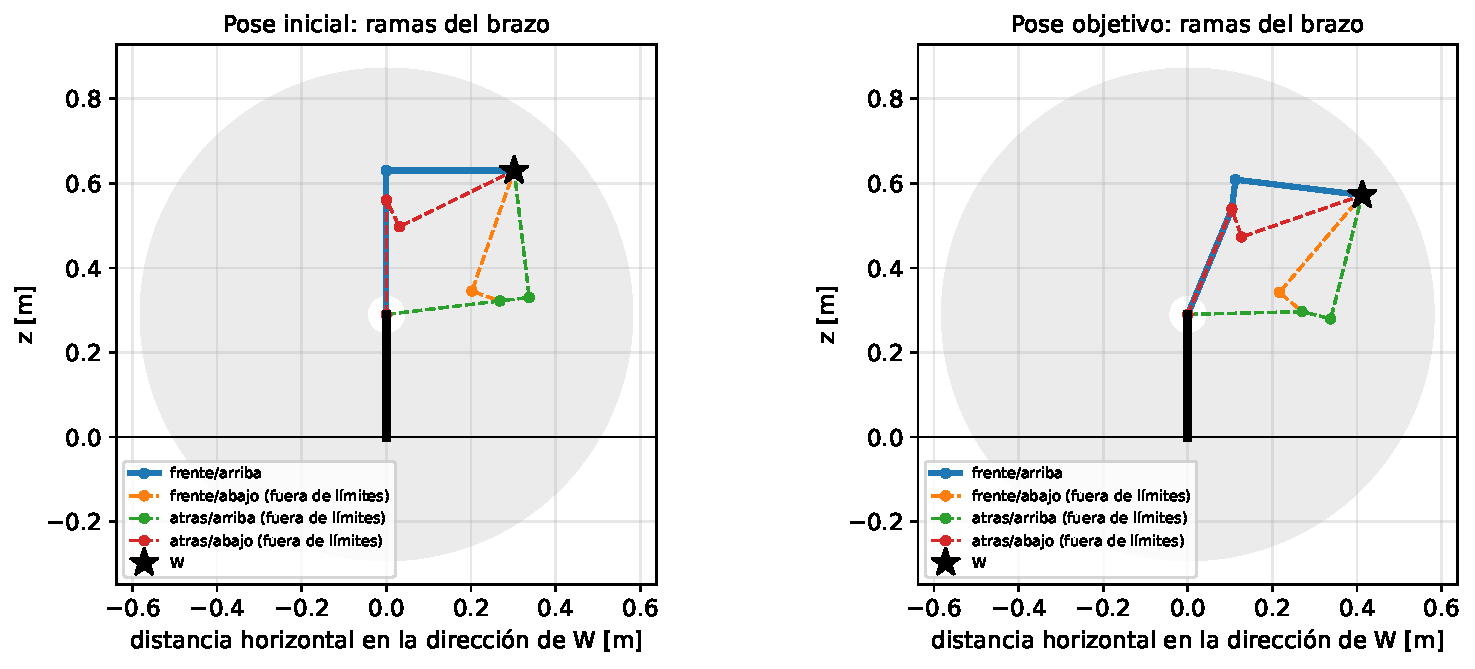
\includegraphics[width=0.82\textwidth]{A_ramas_brazo.pdf}
\caption{Ramas del brazo en el plano de $W$ (hombro, codo, desfase $a_3$ y $W$). En línea continua, las ramas con al
menos una solución admisible; en línea discontinua, las que violan límites. Izquierda: pose inicial. Derecha: pose
objetivo.}
\label{fig:ramas}
\end{figure*}

\subsection{Trayectoria LSPB}
Con la rama elegida,
$\mathbf{q}_f = (\QfDeg)^\circ$. La junta crítica es la \JuntaCritica, que fija $t_f = \Tf$~s con $t_b = \Tb$~s
(Tabla~\ref{tab:lspb}); cuando una misma junta satura velocidad y aceleración, $t_b = v_{\max}/a_{\max}$ y
$t_f = D/v_{\max} + t_b$. Los perfiles (Fig.~\ref{fig:lspb}) cumplen
$\mathbf{q}(0) = \mathbf{q}_0$, $\mathbf{q}(t_f) = \mathbf{q}_f$ y $\dot{\mathbf{q}}(0) = \dot{\mathbf{q}}(t_f) = \mathbf{0}$. Los
saltos de $\mathbf{q}$ y $\dot{\mathbf{q}}$ en los empalmes son a lo sumo $\SaltoMax$, y las seis juntas respetan
$v_{\max}$ y $a_{\max}$.

\begin{table}[t]
\centering
\caption{Parámetros del LSPB ($t_f = \Tf$~s, $t_b = \Tb$~s)}
\label{tab:lspb}
\small
\begin{tabular}{@{}crrrcc@{}}
\toprule
Junta & $D$ [$^\circ$] & $V$ [$^\circ$/s] & $a$ [$^\circ$/s$^2$] & $|V|/v_{\max}$ & $|a|/a_{\max}$\\
\midrule
\tabinput{\resdir/tabla_lspb.tex}
\bottomrule
\end{tabular}
\end{table}

\begin{figure*}[t]
\centering
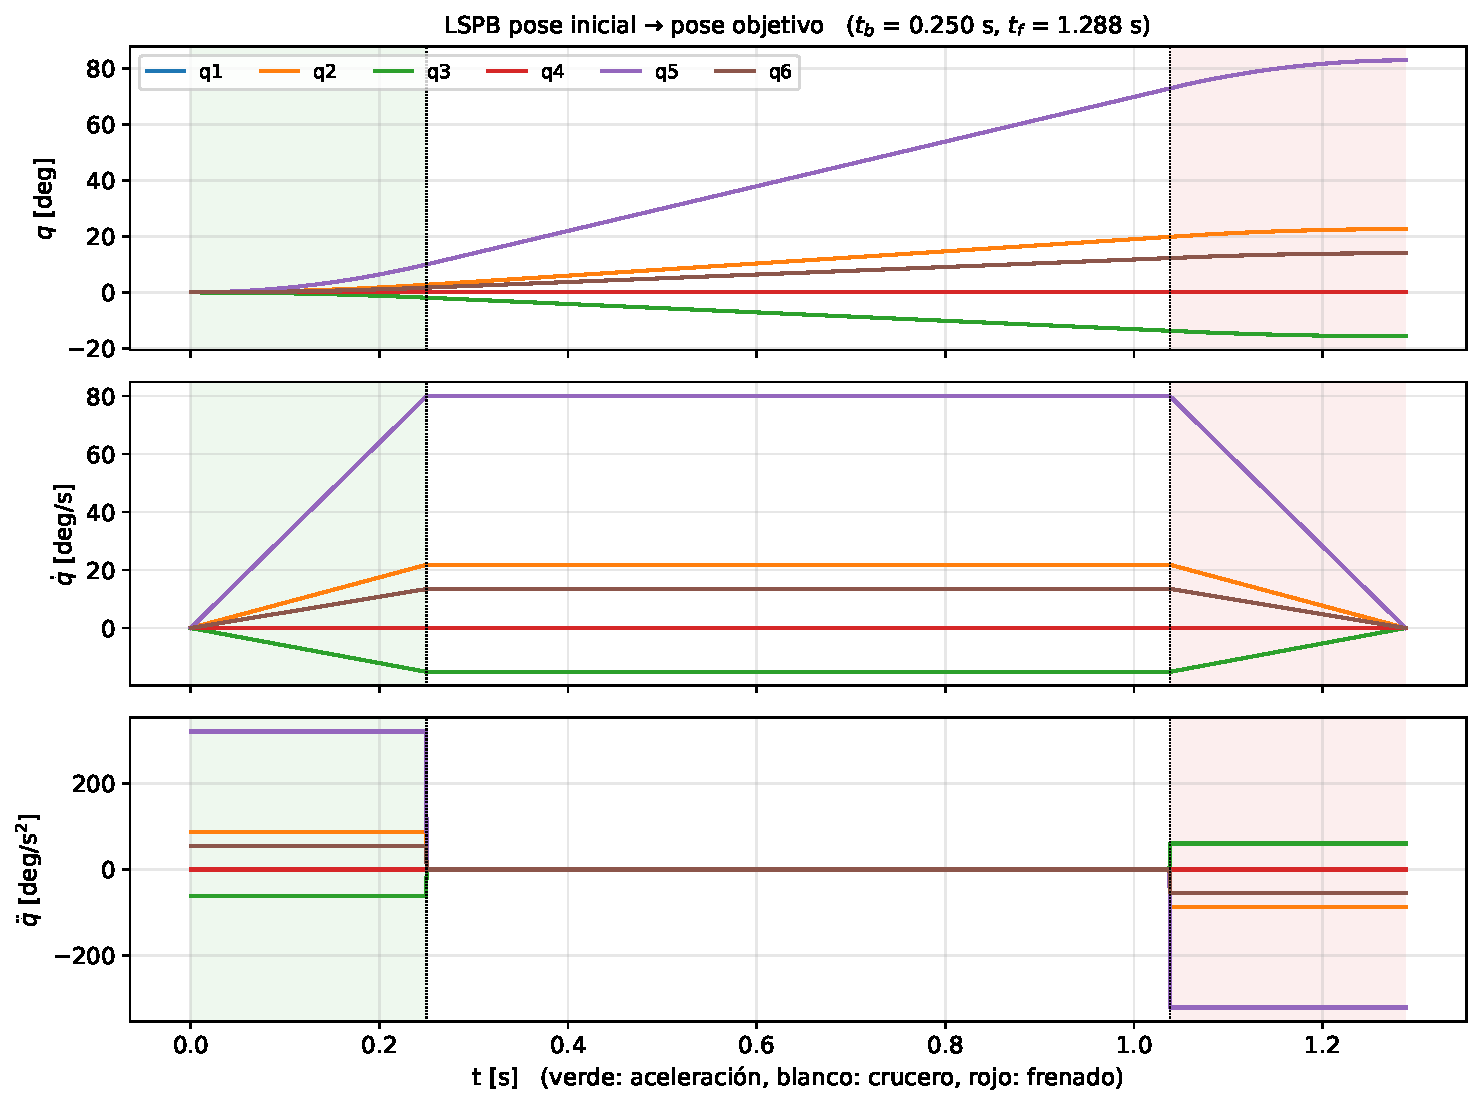
\includegraphics[width=0.68\textwidth]{C_lspb_perfiles.pdf}
\caption{Perfiles LSPB sincronizados $q(t)$, $\dot q(t)$ y $\ddot q(t)$. En verde, la fase de aceleración; en blanco,
el crucero; en rojo, el frenado.}
\label{fig:lspb}
\end{figure*}

\subsection{Jacobiano y singularidad}
El Jacobiano analítico coincide con el numérico con un error de $\ErrJ$, y $J_v\dot{\mathbf{q}}$ coincide con
$d\mathbf{p}/dt$ a lo largo de la trayectoria con un error de $\ErrV$~m/s. En $\mathbf{q} = \mathbf{0}$, las
columnas 4 y 6 son idénticas, $[\mathbf{0};(1,0,0)]$, y el rango es 5: la postura de calibración es singular. En
$\mathbf{q}_f$ el rango es \RangoQf, con $\sigma_{\min} = \SigmaMinQf$. En el experimento de aproximación
(Tabla~\ref{tab:sing}, Fig.~\ref{fig:sing}), solo $\sigma_6$ decrece, con $\sigma_6/\sin q_5 \approx 0.150$. El rango
baja de 6 a 5 exactamente en $q_5 = 0$, y $\det J$ coincide con~\eqref{eq:det}.

En $q_5 = 0$, el espacio nulo de $J$ es $\dot{\mathbf{q}} \propto (0,0,0,1,0,-1)$: un giro opuesto de las juntas 4 y
6 que no mueve el TCP. La dirección perdida (con $W$ como punto de referencia) tiene su componente angular paralela a
$\mathbf{z}_3\times\mathbf{z}_4$, de modo que se pierde una rotación. Para generar un twist unitario en esa dirección
se requiere $\lVert\dot{\mathbf{q}}\rVert = 1/\sigma_6$, con pendiente $-1.000$ en escala log-log. Comparando junta
por junta con el datasheet, $\rho = \max_i|\dot q_i|/v_{\max,i}$: en $q_5 = 0.01^\circ$, las juntas 4 y 6 deberían
girar a $\pm\AmpQdMax$~rad/s, es decir, $\rho \approx \AmpRatio$. Los valores $\sigma_i$ y la tolerancia de rango están en
unidades SI (metros); el rango no depende de esa escala. En cambio, el torque estático
$\lVert J^T\mathbf{u}_6\rVert = \sigma_6$ \emph{tiende a cero}. También se verificó la singularidad de codo en
$q_3 = \delta - 90^\circ = -76.95^\circ$, donde $D \to L_2 + L_3$.

\begin{table}[t]
\centering
\caption{Experimento de aproximación a $q_5 = 0$}
\label{tab:sing}
\small
\begin{tabular}{@{}rcccc@{}}
\toprule
$q_5$ [$^\circ$] & rango & $\sigma_6$ & $\kappa(J)$ & $\lVert\dot{\mathbf q}\rVert$ [rad/s]\\
\midrule
30 & 6 & $7.30\times10^{-2}$ & $2.5\times10^{1}$ & 13.7\\
10 & 6 & $2.58\times10^{-2}$ & $7.0\times10^{1}$ & 38.7\\
1 & 6 & $2.61\times10^{-3}$ & $6.9\times10^{2}$ & 383\\
0.1 & 6 & $2.61\times10^{-4}$ & $6.9\times10^{3}$ & 3824\\
0.01 & 6 & $2.62\times10^{-5}$ & $6.9\times10^{4}$ & 38241\\
0 & \textbf{5} & $1.4\times10^{-17}$ & $\infty$ & ---\\
\bottomrule
\end{tabular}\\[2pt]
{\scriptsize $\lVert\dot{\mathbf q}\rVert$ para un twist unitario en la dirección más débil $\mathbf{u}_6$.}
\end{table}

\begin{figure*}[t]
\centering
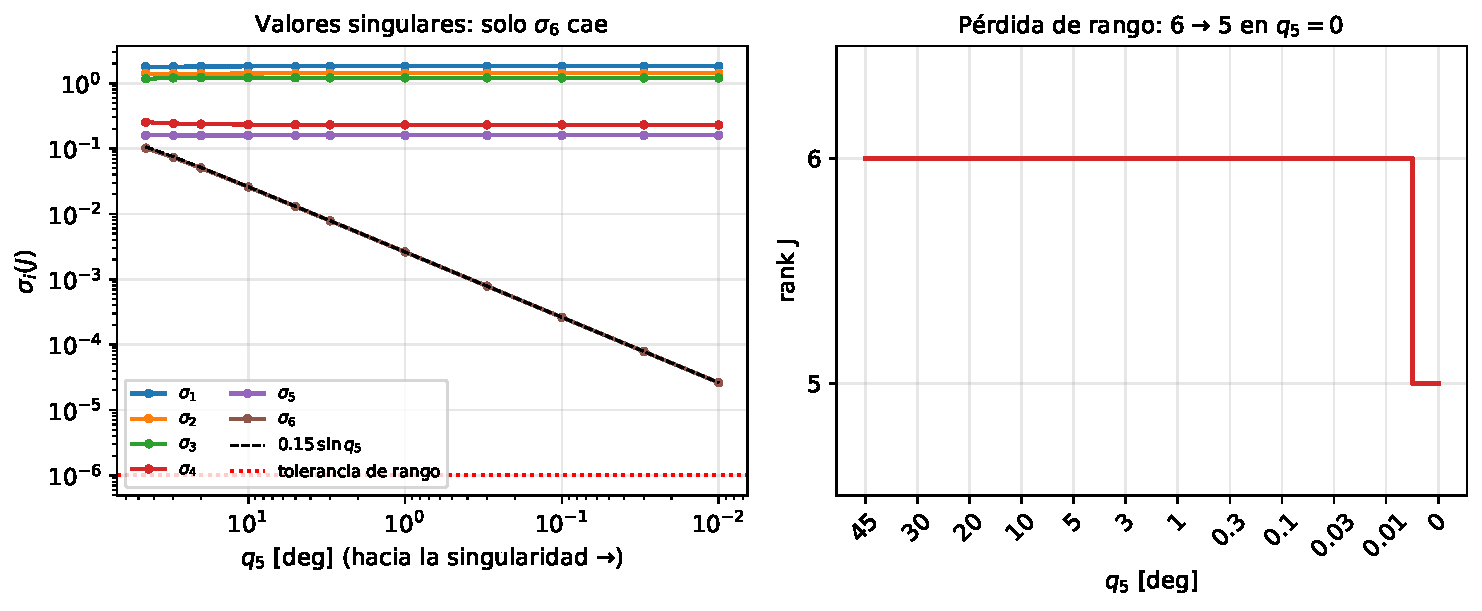
\includegraphics[width=0.8\textwidth]{D_singularidad_rango.pdf}\\[2pt]
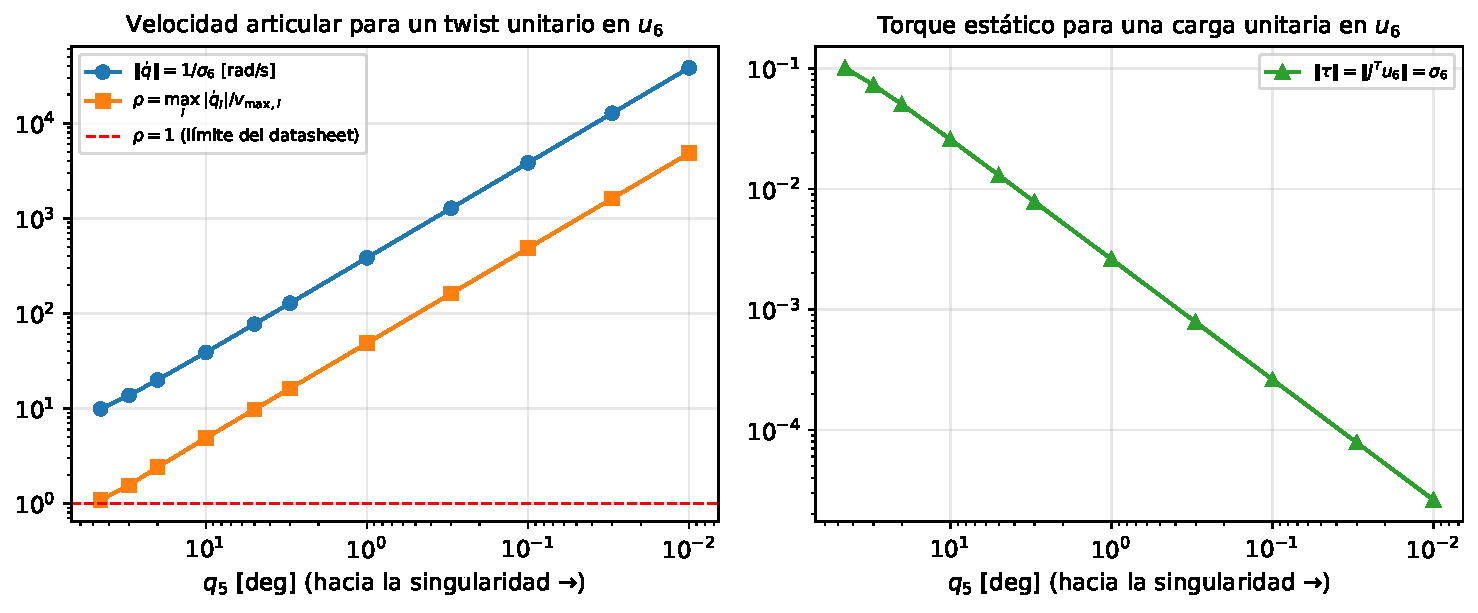
\includegraphics[width=0.8\textwidth]{D_amplificacion.pdf}
\caption{Arriba: valores singulares y rango de $J$ al aproximarse a $q_5 = 0$. Abajo: la velocidad articular para un
twist unitario en la dirección perdida diverge como $1/\sin q_5$ (también comparada junta por junta con el datasheet,
$\rho$), mientras que el torque estático necesario en esa dirección tiende a cero.}
\label{fig:sing}
\end{figure*}

\subsection{Torque del hombro (modelo 1R)}
Los parámetros calculados son $m = \Masa$~kg, $\ell_c = \Lc$~m, $I_c = \Ic$~kg\,m$^2$,
$J = \Jsh$~kg\,m$^2$ y $\varphi_0 = \PhiZero^\circ$, con lo que $mg\ell_c = \MGLc$~N\,m. En $\mathbf{q}_{\text{ref}}$
coinciden exactamente con el modelo de Lagrange completo: $J = M_{22}$ y $\tau_g = g_2$, con diferencias de
$\ErrModelo$. La Tabla~\ref{tab:tau} y la Fig.~\ref{fig:tau} muestran $\tau(t)$. A lo largo de toda la trayectoria, el
1R aproxima el $\tau_2$ del modelo completo de 6~GDL con un error RMS de \RMS~N\,m (\RMSPct\,\%), y un máximo de
\ErrMax~N\,m (Fig.~\ref{fig:val}). Ambos modelos usan los mismos parámetros CAD: la comparación cuantifica la pérdida
por la reducción a 1R, no la fidelidad respecto del robot real, del que no se midieron torques. Al detenerse, el torque
pasa del valor de frenado ($t_f^-$) al de sostén, $\tau = \tau_g = \TauSosten$~N\,m ($t_f^+$).

\begin{table}[t]
\centering
\caption{Torque del hombro en instantes característicos [N\,m]. $t_f^-$: último instante del frenado; $t_f^+$:
robot detenido (solo sostén)}
\label{tab:tau}
\small
\begin{tabular}{@{}rlrrrr@{}}
\toprule
$t$ [s] & Fase & $\theta$ [$^\circ$] & $\tau_{in}$ & $\tau_g$ & $\tau$\\
\midrule
\tabinput{\resdir/tabla_torque.tex}
\bottomrule
\end{tabular}
\end{table}

\begin{figure*}[t]
\centering
\begin{minipage}[b]{0.55\textwidth}\centering
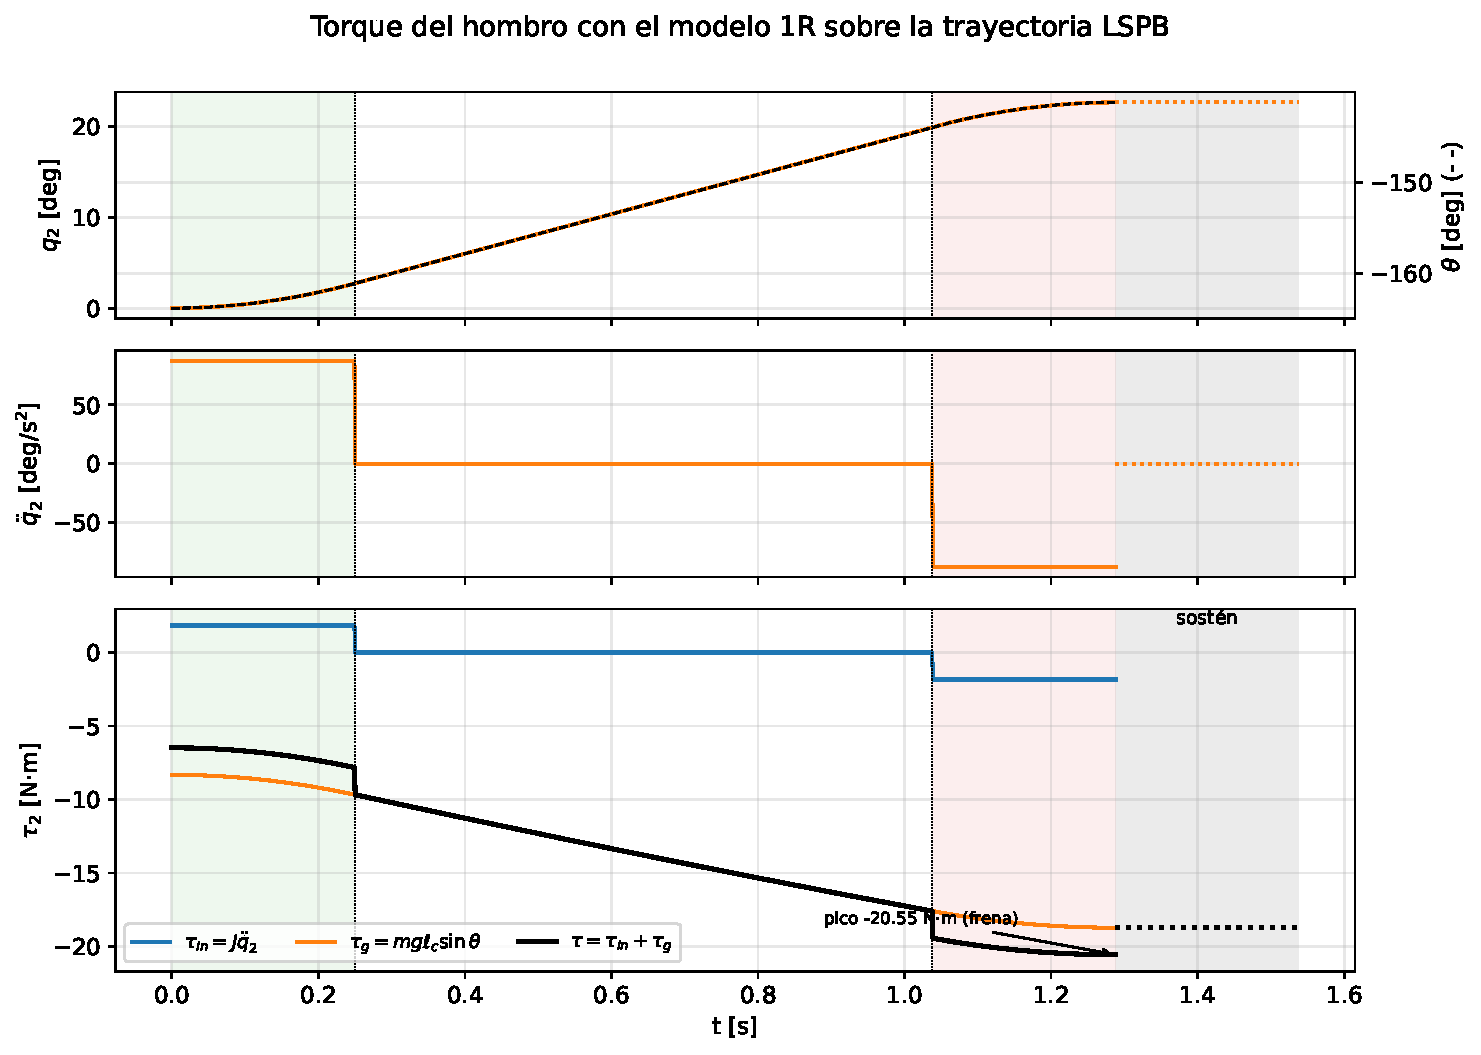
\includegraphics[width=\linewidth]{E_torque_1R.pdf}
\caption{Modelo 1R del hombro: $q_2$ (y $\theta$), $\ddot q_2$ y $\tau = \tau_{in} + \tau_g$ sobre el LSPB, más
0.25~s de sostén (gris) con el robot detenido.}
\label{fig:tau}
\end{minipage}\hfill
\begin{minipage}[b]{0.42\textwidth}\centering
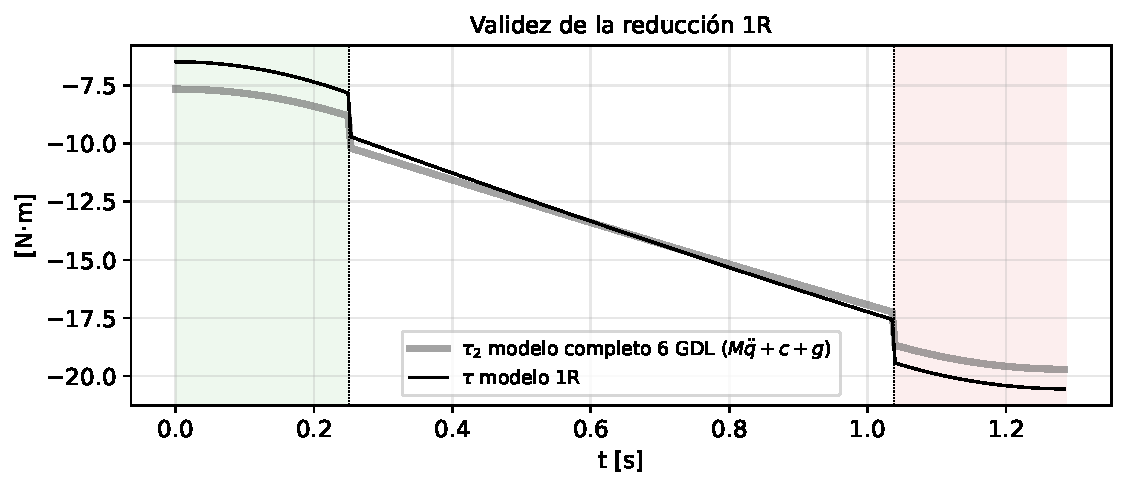
\includegraphics[width=\linewidth]{E_1R_vs_completo.pdf}
\caption{Torque del hombro: modelo 1R frente al modelo de Lagrange completo de 6~GDL (mismos parámetros CAD).}
\label{fig:val}
\end{minipage}
\end{figure*}

% =====================================================================================================
\section{Discusión}
\textbf{Aceleración frente a crucero.} La componente inercial $\tau_{in} = J\ddot q_2$ solo existe en las mezclas y
presenta escalones, porque $\ddot q$ en el LSPB es discontinua: el perfil es $C^1$, no $C^2$. Donde $\tau_{in}$ y
$\tau_g$ tienen signos opuestos, el torque neto es menor que el estático (en $t = 0$, $\tau = \TauIni$~N\,m); donde
tienen el mismo signo se suman, y ahí aparece el pico de $\TauPeak$~N\,m (fase: \TauPeakFase, $t = \TauPeakT$~s).
% REVISAR si cambia la pose: confirmar en qué fase cae el pico (lo imprime el notebook, sección 9.1).
Durante el crucero, $\ddot q_2 = 0$ y aun así $|\tau|$ va de \CruceroRango~N\,m: \emph{velocidad constante no implica
torque cero}, porque el motor sostiene el peso. Con $\theta$ cerca de $\pm180^\circ$, el centro de masa está por encima
del eje y el brazo se comporta como un péndulo invertido: alejarse de la vertical aumenta $|\sin\theta|$ y con ello el
esfuerzo. Al 25\,\% de velocidad domina la gravedad ($\max|\tau_{in}| = \TauInMax$ frente a
$\max|\tau_g| = \TauGMax$~N\,m). Si la misma trayectoria se recorre $\lambda$ veces más rápido, $\tau_{in}$ crece como
$\lambda^2$: al 100\,\% alcanza \TauInFull~N\,m, mientras que $\tau_g$ (\TauGFull~N\,m) no cambia.

\textbf{Singularidad frente a pico de torque.} La singularidad es una propiedad cinemática de la postura: $J$ pierde
rango y desaparece una dirección de movimiento instantáneo. Lo que diverge es la velocidad articular necesaria para
moverse en esa dirección. Por estática ($\tau = J^TF$), una carga en la dirección perdida no requiere torque. El pico de
torque, en cambio, es un fenómeno dinámico: depende de la aceleración impuesta por el perfil temporal y de la
gravedad. En este caso, la trayectoria \emph{parte} de una singularidad ($\mathbf{q}_0 = \mathbf{0}$) sin dificultad,
porque el LSPB es articular y no invierte $J$. El pico de torque ocurre en la fase de \TauPeakFase, lejos de esa
singularidad. % REVISAR si cambia la pose: rango de J en el pico (sección 9.1 del notebook).

\textbf{Limitaciones.} El modelo 1R congela las juntas 3 a 6 y omite la fricción, la carga útil y el acoplamiento entre
juntas. Como su inercia $J$ es constante, no tiene término en $\dot\theta^2$; un modelo con inercia dependiente de la
postura sí lo tendría. Su error frente al modelo completo es mayor al principio y al final del movimiento, donde la postura real se
aleja de $\mathbf{q}_{\text{ref}}$. El valor de $a_{\max}$ es un supuesto, porque el fabricante no lo publica.

% =====================================================================================================
\section{Conclusiones}
Se validó un pipeline completo para el ABB IRB~120, desde la posición de calibración hasta una pose objetivo
arbitraria. La cinemática inversa analítica de Pieper enumera las ocho ramas, distingue las reales de las admisibles y
cada candidato se verifica por FK con errores del orden de la precisión de máquina. El LSPB sincronizado de tiempo
mínimo cumple las fronteras en reposo y los límites del fabricante. El Jacobiano, validado de forma independiente,
permitió caracterizar la singularidad de muñeca por la pérdida de rango y explicar su efecto: amplificación de
velocidad, no torque infinito. Finalmente, el modelo 1R del hombro, con parámetros obtenidos de datos CAD, separa las
contribuciones inercial y gravitacional y reproduce al modelo completo con un \RMSPct\,\% de error RMS. La solución de
posición resulta ser el requisito sobre el cual operan los análisis de sensibilidad diferencial y de demanda de los
actuadores.

\begin{thebibliography}{00}
\bibitem{siciliano} B. Siciliano, L. Sciavicco, L. Villani, and G. Oriolo, \textit{Robotics: Modelling, Planning and
Control}. London, U.K.: Springer, 2009.
\bibitem{pieper} D. L. Pieper, ``The kinematics of manipulators under computer control,'' Ph.D. dissertation, Dept.
Mech. Eng., Stanford Univ., Stanford, CA, USA, 1968.
\bibitem{bahani} A. Bahani, M. E. Ech-Chhibat, H. Samri, and H. Ait Elattar, ``The inverse kinematics evaluation of
6-DOF robots in cooperative tasks using virtual modeling design and artificial intelligence tools,''
\textit{Int. J. Mech. Eng. Robot. Res.}, vol.~12, no.~2, pp.~121--130, Mar. 2023, doi: 10.18178/ijmerr.12.2.121-130.
\bibitem{truc} L. N. Truc and N. T. Lam, ``Quasi-physical modeling of robot IRB 120 using Simscape Multibody for
dynamic and control simulation,'' \textit{Turk. J. Elec. Eng. \& Comp. Sci.}, vol.~28, pp.~1949--1964, 2020,
doi: 10.3906/elk-1909-131.
\bibitem{abb} ABB Robotics, \textit{Product Specification IRB 120}, doc. 3HAC035960-001.
\bibitem{abbcal} ABB Robotics Tech Community, ``Calibrate an IRB140'' (actualización de contadores de revolución con
\texttt{MoveAbsJ} a un \textit{jointtarget} de ceros), 2014. [En línea]. Disponible:
\url{https://tech-community.robotics.abb.com/t/calibrate-an-irb140/4976}
\bibitem{rosi} ROS-Industrial, ``abb\_irb120\_support: irb120\_3\_58\_macro.xacro,'' paquete \textit{abb}, rama
kinetic-devel. [En línea]. Disponible: \url{https://github.com/ros-industrial/abb/tree/kinetic-devel/abb_irb120_support}
\bibitem{guia} B. Quiroga, ``Guía oficial y rúbrica de evaluación: Hito 2,'' IMT-342 Robótica, Universidad Católica
Boliviana, Tarija, 2026.
\end{thebibliography}

\end{document}
